% 0. Preamble: -----------------------------------------------------{{{
% 0.1 Document Class Setup: ----------------------------------------{{{

\documentclass[12pt]{article}

%}}}
% 0.2 Packages + Libraries: ----------------------------------------{{{

\usepackage{amsfonts, array, amsmath, amssymb, bm, caption, booktabs, mathtools, tikz}
\usepackage[margin=0.21in]{geometry}
\usepackage[]{microtype}
\usetikzlibrary{shapes.geometric,arrows,positioning,fit, calc}

%}}}
% 0.3 Commands: ----------------------------------------------------{{{

% binomial exponents - 3 args, 1st arg 2
\newcommand{\negBi}[3][2]{{(#2- #3)}^{#1}}
\newcommand{\negBiBold}[3][2]{\bm{{(#2- #3)}^{#1}} }

%}}}
%}}}
\begin{document}
% Section: Conditions for a z-test about a proportion ---------------{{{
\section*{Conditions for a z-test About a Proportion:}
% Subsection: Scenario ------------------------------{{{
\subsection*{Scenario}
Jules is on a team of 40 employees. Each employee gets an annual rating, the best is ``exceeds expectation.'' Management \textbf{claimed that 10\% of employees} get this rating, Jules \textbf{suspected it was actually less common}. She got an anonymous random sample of 10 ratings for employees on her team. She wants to use the sample data to test $H_{0}$: $p=0.1$ vs. $H_{a}$: $p < 0.1$, where $p$ is the proportion of all employees on her team who ``exceeds expectation.''
%}}}
% Subsection: Hypotheses ------------------------------{{{
\subsection*{Hypotheses}
\begin{align}
  \text{The null hypothesis is based on the claim itself:} &&
  H_{0}: \; p = 0.10 \\
  \text{The alternative hypothesis is based on what is suspected:} &&
  H_{a}: \; p < 0.10
\end{align}
%}}}
% Subsection: Visualize ------------------------------{{{
% Using tikzpicture positioning library
\subsection*{Visualize}
\begin{center}
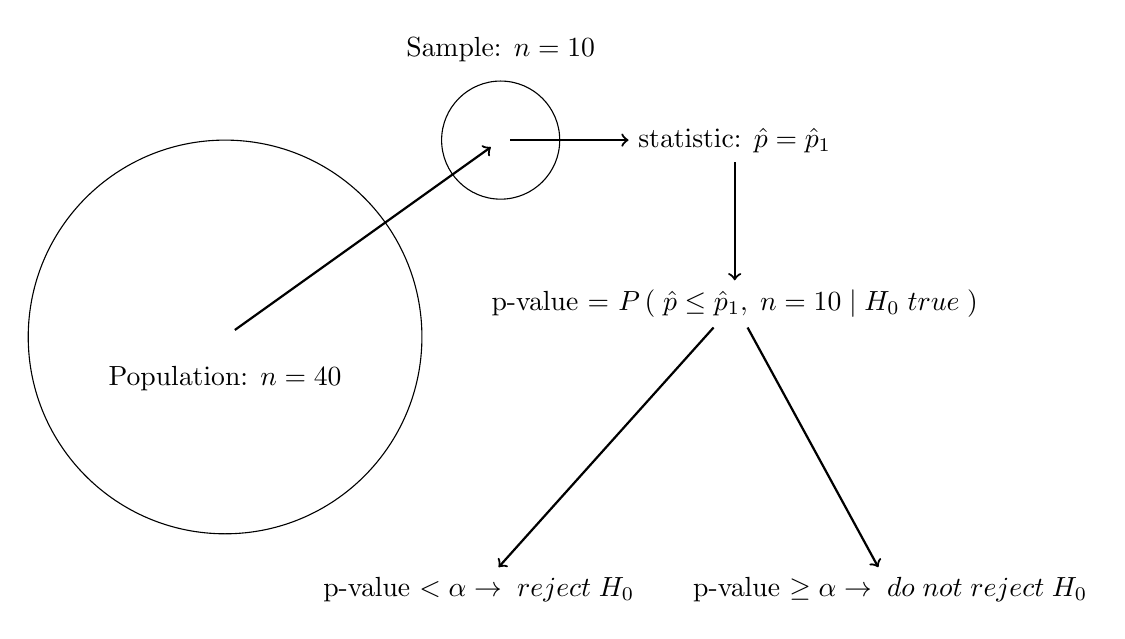
\begin{tikzpicture}
  \draw [fill=white] (0,0) circle (2.5cm)
      node (population) {};
  \node (poplabel)[below = 0.25]{Population: $n=40$};
  \draw [fill=white] (3.5,2.5) circle (0.75cm)
      node (sample) {};
  \node (samplabel) [above = 0.75 of sample]{Sample: $n=10$};
  \node (statlabel) [right = 1.5 of sample]{statistic: $\hat{p}=\hat{p}_{1}$};
  \node (pvalueequation) [below = 1.5 of statlabel]
    {p-value = $
      P\left(\;\hat{p} \le \hat{p}_{1},\;n = 10 \mid H_{0} \; true\;\right)
    $};
  \node (pvaluelow) [below right = 2.8cm and 1cm of population]
    {p-value $< \alpha \rightarrow \; reject \; H_{0}$};
  \node (pvaluehigh) [right = 0.5cm of pvaluelow]
    {p-value $\ge \alpha \rightarrow \; do \; not \; reject \; H_{0}$};
  % Draw arrows
  \draw[->, thick, to path={-- (\tikztotarget)}]
    (population) edge (sample);
  \draw[->, thick, to path={-- (\tikztotarget)}]
    (sample) edge (statlabel);
  \draw[->, thick, to path={-- (\tikztotarget)}]
    (statlabel) edge (pvalueequation);
  \draw[->, thick, to path={-- (\tikztotarget)}]
    (pvalueequation) edge (pvaluelow);
  \draw[->, thick, to path={-- (\tikztotarget)}]
    (pvalueequation) edge (pvaluehigh);
\end{tikzpicture}
\end{center}
%}}}
% Subsection: Description ------------------------------{{{
\subsection*{Description}
\begin{itemize}
  \item From the population (40 employees), take a sample (10 employees), then calculate a sample statistic \textbf{(sample proportion)} and assign it to $\bm{\hat{p}_{1}}$.
  \item Next calculate a p-value, remembering that a \textbf{p-value is the probability of getting a result at least as extreme, if we assume the null hypothesis is true}. Because Jules suspects that 10\% are not exceeding expectations, this is the probability that the sample statistic is less than or equal to the one, that was calculated for the sample size (n = 10), given the null hypothesis is true.
  \item If the \textbf{p-value is less} than the predetermined significance level then the null hypothesis is rejected. If the \textbf{p-value is not less} than the significance level, then the null hypothesis can not be rejected.
\end{itemize}
%}}}
% Subsection: Conditions Check ------------------------------{{{
\subsection*{Conditions Check}
\begin{itemize}
  \item \textbf{Random}: Yes. \textbf{``obtained an anonymous random sample''} is explicit in description.
  \item \textbf{Normal}: No. Successes and Failures must be at least equal to 10 $\bm{(np, \; n(1-p) \ge 10)}$. In this case (n = 10 and p = 0.1): $\bm{(10*0.1=1 \;and\; 10*0.9=9)}$, so this condition is not satisfied.
  \item \textbf{Independence}: No. Jules is \textbf{not using replacement} and \textbf{sample size is not less than 10\%} of the population. $\bm{(10/40=0.25)}$
\end{itemize}
%}}}
%}}}
\end{document}
